\documentclass[11pt]{article}
\usepackage[margin=1in]{geometry}
\usepackage{jheppub} % for details on the use of the package, please see the JINST-author-manual
% page formatting
\usepackage{fancyhdr}
\pagestyle{fancy}

\renewcommand{\sectionmark}[1]{\markright{\textsf{#1}}}
\renewcommand{\subsectionmark}[1]{}
\lhead{\textbf{\thepage} \ \ \nouppercase{\rightmark}}
\chead{}
\rhead{}
\lfoot{}
\cfoot{}
\rfoot{}
\setlength{\headheight}{14pt}

\linespread{1.03} % give a little extra room
\setlength{\parindent}{0.2in} % reduce paragraph indent a bit
\setcounter{secnumdepth}{2} % no numbered subsubsections
\setcounter{tocdepth}{2} % no subsubsections in ToC
\usepackage{lineno}
\usepackage{amsmath,amsthm,amsfonts,amssymb,amscd,physics,cancel,mathtools}
\usepackage{tcolorbox}
\usepackage{marginnote,tensor}
\usepackage[spanish]{babel}
%~~~~~~~~~ Document setup
% \usepackage[spanish]{babel} % English formatting
\usepackage[utf8]{inputenc} % Standard encoding
% \usepackage[a4paper,left=3cm,bottom=3cm]{geometry} % Page formatting
\usepackage{indentfirst} % Indents the first paragraph
\usepackage{amsmath} % Maths type package
\usepackage{bm} % Bold font maths
\usepackage{graphicx} % Advanced graphics package
\usepackage[export]{adjustbox} 
\usepackage{pdflscape} % Make pages landscape
\usepackage{fancyhdr} % Fancy headers
% \usepackage[colorlinks=true,citecolor=blue,urlcolor=blue,linkcolor=black]{hyperref} % Link colours
%\usepackage{natbib} % Bibliography
% \usepackage{flafter} % Reference any 'float'
% \usepackage[framemethod=tikz]{mdframed} % Box off stuff
\usepackage{color} % Colour support
\usepackage{wrapfig} % Text flowing around figures
\usepackage{lipsum} % Generates meaningless text
\usepackage{xcolor}
\usepackage{wrapfig}
%\usepackage{biblatex}
%\usepackage[backend=bibtex]{biblatex}
%\addbibresource{bibliography.bib}
%\hypersetup{colorlinks=true, linkcolor=blue}


\theoremstyle{definition}
\newtheorem{ej}{Ejemplo}[section]
\newtheorem{teor}{Teorema}[section]
\newtheorem{sol}{Solución}[section]
\newtheorem{dem}{Demostración}[section]
\newtheorem{cor}{Corolario}[section]
\newtheorem{post}{Postulado}
\newtheorem{prop}{Propiedad}[section]
\newtheorem{prueba}{Prueba}[section]
\newtheorem{Propo}{Proposición}[section]
\newtheorem{defi}{Definición}[section]


\def\a{\alpha}
\def\b{\beta}
\def\g{\gamma}
\def\G{\Gamma}
\def\d{\delta}
%\def\D{\Delta}
%\def\e{\eta}
\def\la{\lambda}
\def\La{\Lambda}
\def\k{\kappa}
\def\m{\mu}
\def\n{\nu}
\def\r{\rho}
\def\p{\rho}
\def\o{\omega}
\def\s{\sigma}
\def\S{\Sigma}
\def\t{\tau}
\def\p{\pi}
\def\f{\phi}
\def\vf{\varphi}
\def\ep{\epsilon}
\def\th{\theta}
\def\Th{\Theta}
\def\z{\zeta}
\def\zc{Z_{\rm C}}
\def\zgc{Z_{\rm GC}}
\def\zp{Z_{p}}
\def\ogc{\omega_{\rm GC}}
\def\Ogc{\Omega_{\rm GC}}
\def\dst{\dd S_{\rm total}}
\def\vec{\vb*}
\def\eb{e^{-\beta E_i}}
\def\ebep{e^{-\beta \epsilon_i}}
\def\eba{e^{-\beta E_i-\alpha Q_i}}
\def\ebaj{e^{-\beta E_j-\alpha Q_j}}
\newcommand{\summ}{\sum_{i=1}^m}
\newcommand{\sumi}{\sum_i}
\newcommand{\sumj}{\sum_j}
\def\var{\text{Var}}
\def\intpq{\int\frac{\dd^3\vec{p}\dd^3\vec{q}}{(2\pi\hbar)^3}}
\def \sumn1 {\sum_{n=1}^\infty}
\def\ebem{e^{-\b (\ep-\m )}}
\def\qd{\dot{q}}


%-----COLORS LIST ------
\definecolor{azure(colorwheel)}{rgb}{0.0, 0.5, 1.0}
\definecolor{DarkViolet}{RGB}{148,0,211}
\definecolor{myDarkBlue}{rgb}{0,0.1,0.7}
\definecolor{DarkBlue}{RGB}{0,0,153}
\definecolor{amber}{rgb}{1.0, 0.49, 0.0}
\definecolor{amaranth}{rgb}{0.9, 0.17, 0.31}
\definecolor{nicered}{rgb}{0.7,0.1,0.1}
\definecolor{brown}{rgb}{0.5,0.1,0.1}
\definecolor{nicegreen}{rgb}{0.0,0.3,0.0}
\definecolor{tealgreen}{rgb}{0.0, 0.51, 0.5}
\def\red#1{{\color{red} #1}}
\def\green#1{{\color{green} #1}}
\def\blue#1{{\color{blue} #1}}
\def\orange#1{{\color{orange} #1}}
%----------------------
\newcommand{\mycolor}{DarkViolet}
\def\myColor#1{{\color{\mycolor} #1}}
\definecolor{tclr}{RGB}{148,0,211}
%----------------------
\newcommand{\corr}[1]{\textcolor{nicered}{#1}}
\newcommand{\nick}[1]{\textcolor{olive}{#1}}
\newcommand{\teo}[1]{\textcolor{azure(colorwheel)}{#1}}
\newcommand{\chteo}[2]{\corr{\st{#1}} \teo{(#2)}}
\newcommand{\bako}[1]{\textcolor{DarkViolet}{#1}}
\newcommand{\than}[1]{\textcolor{magenta}{#1}}
%----------------------
\usepackage{hyperref}
\hypersetup{colorlinks,bookmarksopen,
	bookmarksnumbered,
	citecolor={nicered},
	linkcolor={myDarkBlue},
	urlcolor={blue},
	pdfstartview=FitH}





% \arxivnumber{1234.56789} % if you have one

%\title{\boldmath Mecánica Estadística}

% Collaborations

%% [A] If main author
%% \collaboration{\includegraphics[height=17mm]{collabroation-logo}\\[6pt]
%%  XXX collaboration}

%% or
%% [B] If "on behalf of"
%% \collaboration[c]{on behalf of XXX collaboration}


% Authors
% The "\note" macro will give a warning: "Ignoring empty anchor...", you can safely ignore it.

%% [A] simple case: 2 authors, same institution
%% \author[1]{A. Uthor\note{Corresponding author.}}
%% \author{and A. Nother Author}
%% \affiliation{Institution,\\Address, Country}

%% or, e.g.
%% [B] more complex case: 4 authors, 3 institutions, 2 footnotes
%% \author[a,b]{F. Irst,\note{Now at another university}}
%% \author[c]{S. Econd,}
%% \author[a,2]{T. Hird\note{Also at Some University.}}
%% \author[c,2]{and Fourth}
%% \affiliation[a]{Institution_1,\\Address, Country}
%% \affiliation[b]{Institution_2,\\Address, Country}
%% \affiliation[c]{Institution_3,\\Address, Country}

\author{Borja Diez}
\affiliation{Universidad Arturo Prat}
% \affiliation{Another University,\\
% different-address, Country}

% E-mail addresses: only for the corresponding author
\emailAdd{borjadiez1014@gmail.com}

\abstract{Notas sobre Mecánica Estadistica }



\begin{document}
% make title page
\thispagestyle{empty}
\bigskip \
\vspace{0.1cm}

\begin{center}
{\fontsize{22}{22} \selectfont Notas de Clase en}
\vskip 16pt
{\fontsize{36}{36} \selectfont \bf \sffamily Lagrangeanos singulares y Hamiltonianos con vínculos}
\vskip 24pt
{\fontsize{18}{18} \selectfont \rmfamily Borja Diez} 
\vskip 6pt
{\fontsize{14}{14} \selectfont \ttfamily borjadiez1014@gmail.com}
\vskip 6pt
{\fontsize{14}{14} \selectfont  \sffamily \today}
\vskip 24pt
\end{center}

Estas notas de clase están basadas en el curso dictado por el \href{https://inspirehep.net/authors/2180313?ui-citation-summary=true}{Dr. Luis Avilés} durante el primer semestre del año 2024 en la Universidad Arturo Prat y han sido escritas con propósito de estudio personal.

Las notas están divididas por clase. Adicionalmente han sido complementadas con desarrollos de cálculo personal .
%y comentarios sacados principalmente de \textcolor{blue}{Lecture notes on statistical mechanics} de \href{https://inspirehep.net/authors/992816}{Scott Pratt}. 

La bibliografía principal es \cite{Henneaux:1994lbw}, \cite{Rothe:2010dzf}, \cite{Saavedra:2000wk} y \cite{Sundermeyer:1982gv}. 




% make table of contents
\newpage
\tableofcontents
\newpage

\section{Clase 1}
%\subsection{Lagrangeanos singulares y Hamiltonianos con vínculos}
Las teorías más exitosas que conocemos poseen simetrías de gauge (electrodínamica y teorías de Yang-Mills). Dichas teorías se caracterizan porque poseen \textit{vínculos}.

Las simétrias de gauge son simetrias que actuan sobre los campos localmente.

Las teorías que possen \textit{simetrías de gauge} son sistemas físicos con \textit{vínculos.}

Una caracteristica que poseen en común estas teorías es que están descritas mediante más variables que grados de libertad físicamente independientes. Por ejemplo, la electrodinámica posee simetría de gauge, por lo tanto un sistema físico puede ser descrito por infinitos campos $A_\m $, pero en realidad la teoría tiene $2$ grados de libertad físicos. Sistemas que tiene esta propiedad son conocidos como \textit{singulares}.


Las ecuaciones de Euler-Lagange incluyen ecuaciones que representan vínculos entre las coordenadas y las velocidades, $\Phi(q_i,\dot{q}_i)=0$. Por lo tanto, no todos los grados de libertad estarán completamente determinados por las ecuaciones. 
%\textit{que la misma dinámica impone en el sistema}
A nivel Hamiltoniano, estas teorías tienen vínculos de \textit{primera clase} los cuales corresponde a los \textit{generadores} de las simetrías de gauge. Es decir, toda teoría de gauge implica una teoría con vínculos, pero el recíproco no es verdad,

\begin{equation}
  \boxed{\text{Teorías de gauge} \implies \text{Teorías con vínculos}}.
\end{equation}


\subsection{Invariancia de gauge y vinculos}
Una teoría de gauge podría ser pensada como una teoría en que las variables dinámicas son especificadas con respecto a un sistema de referencia cuya eleccción es arbitraria para cada instante de tiempo. Las variables físicamente importantes son aquellas que son independientes del sistema de referencia local. Una transformación de las variables inducidas por un cambio arbitrario en el marco de referencia es conocida como una \textit{transformación de gauge}.


\begin{wrapfigure}{r}{0.4\textwidth}
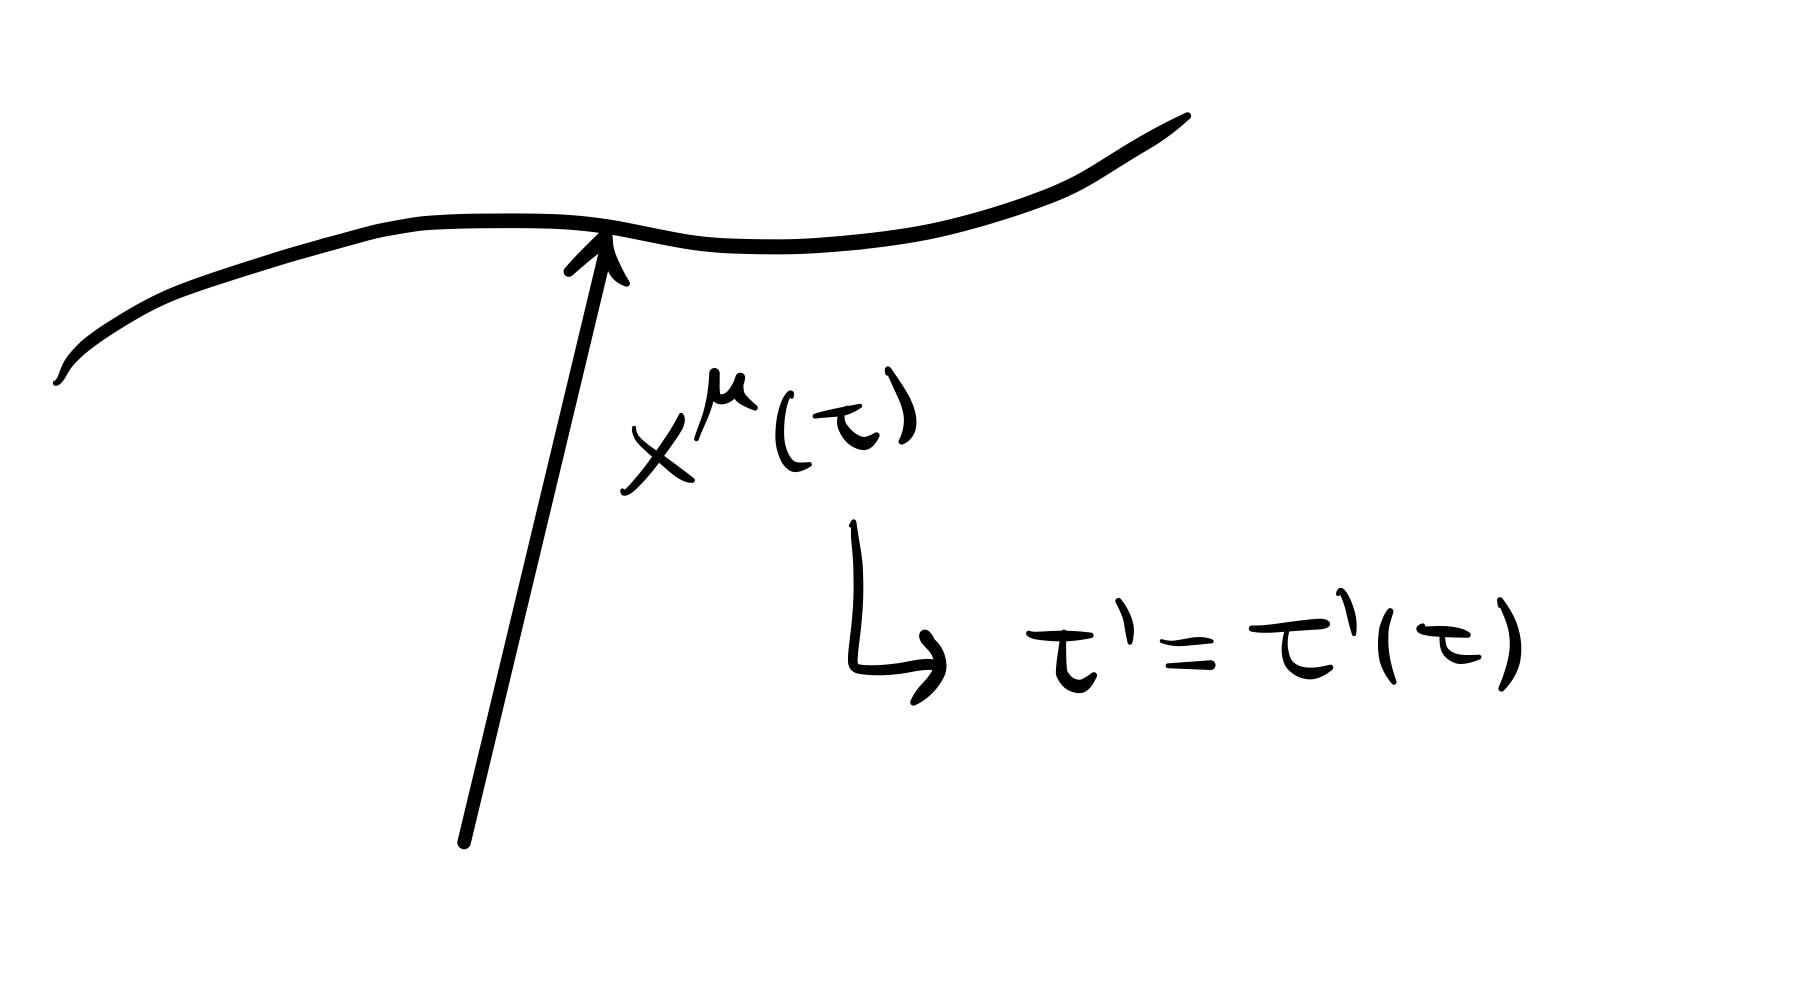
\includegraphics[width=1.0\linewidth]{1-particula} 
\end{wrapfigure}
Las varibles físicas (observables) son aquellas que son invariantes bajo transformaciones de gauge.



\begin{ej}


	Consideremos la trayectoria de una partícula relativista.
	
	En este caso la trayectoria de la partícula $x^\m$ es el campo dinámico, $\t $ es el parámetro propio relacionado con el sistema de referencia y $\t' $ es una reparametrización del parámetro propio.
	
	Consideremos una tranformación infinitesimal
	\begin{equation}
  \t'=\t +\epsilon(\t ),
\end{equation}
la cual induce una transformación de gauge sobre los campos  de la forma
\begin{equation}
  \d x^\m =-\epsilon (\t )\dot{x}^\m,
\end{equation}
y el observable corresponde a la longitud de arco $S$.
\end{ej}


En una teoría de gauge, uno no puede esperar que las ecuaciones de movimiento determinen todas las variables para todo tiempo. A partir de las misma ecuaciones iniciales, se producirán evoluciones temporales diferentes. Por lo tanto, una propiedad clave de una teoría de gauge es que la solución general de las ecuaciones de movimiento contienen funciones arbitrarias del tiempo.

La aparición de funciones arbitrarias en la solución general de las ecuaciones de movimeinto implica, a nivel Hamiltoniano, que las variables canónicas no son todas independientes. La relación que existe entre ellas son llamadas \textit{vínculos},
\begin{equation}
  \Phi(p,q)=0.
\end{equation}

\begin{tcolorbox}
En resumen, en una teoría de gauge
\begin{itemize}
	\item existe una relación entre las ecuaciones,
	\item no todas las variables están fijas por las ecuaciones de movimiento,
	\item existen vínculos de primera clases en el Hamiltoniano.
\end{itemize}
\end{tcolorbox}

\begin{ej}
	Consideremos la siguiente acción:
	\begin{equation}
  I[\psi,A_0]=\frac{1}{2}\int\dd t\left(\dot{\psi}-A_0\right)^2
\end{equation}
\begin{enumerate}
	\item \underline{\textit{Simetría de gauge}}: Esta acción es invariante bajo las siguientes transformaciones,
	\begin{equation}
  \psi'=\psi+\epsilon(t),\qquad A_0=A_0+\dot{\epsilon}(t)
\end{equation}
es directo ver que
\begin{equation}
  \d\psi=\epsilon(t),\quad \d A_0=\dot{\epsilon}(t)
\end{equation}
En efecto, la variación de la acción queda,
\begin{align}
  \d I&=\frac{1}{2}\int\dd t\left(\dv{t}(\d\psi)-\dot{\epsilon}(t)\right)^2\\
  &=\frac{1}{2}\int\dd t\left(\dot{\epsilon}(t)-\dot{\epsilon}(t)\right)^2\\
  &=0
\end{align}
donde $\epsilon(t)$ es arbitrario.

\item \underline{\textit{Las ecuaciones de movimiento no son independientes}}:
\begin{equation}
  \frac{\d I}{\d A_0}=0\implies (\dot{\psi}-A_0)=0
\end{equation}
\begin{equation}
  \frac{\d I}{\d \psi}=0\implies 2\left(\dot{\psi}-A_0\right)\dv{t}(\d\psi)=0\implies \dv{t}(\dot{\psi}-A_0)=0
\end{equation}
Es fácil ver que ambas ecuaciones son diferencialmente dependientes.
\item \underline{\textit{La solución más general contiene funciones arbitrarias}}: La solución más general para este sistema de ecuaciones será,
\begin{align}
  \psi(t)&=f(t)\\
  A_0(t)&=\dot{f}(t)
\end{align}
Por lo tanto, implica una función arbitraria.

Independiente de cuales seal las condiciones iniciales, uno siempre puede modificar la evolución en un tiempo posterior.

\item \underline{\textit{El Hamiltoniano posee vínculos}}. Para pasar a la formulación Hamiltoniana, calculamos las momentas,
\begin{align}
  P_{A_0}&=\pdv{L}{\dot{A_0}}=0\\
  P_{\psi}&=\pdv{L}{\dot{\psi}}=\left(\dot{\psi}-A_0\right)
\end{align}
Luego, el Hamiltoniano queda
\begin{align}
  H&=P_\psi \dot{\psi }-L\\
  &=P_\psi(P_\psi+A_0)-\frac{P_\psi^2}{2}\\
  &=\frac{P_\psi^2}{2}+P_\psi A_0
\end{align}
Escribimos la acción Hamiltoniana
\begin{align}
  I[P_\psi,\psi,A_0]&=\int\left(P_\psi \dot{\psi}-\frac{1}{2}P^2_\psi-A_0P_\psi\right)\dd t
\end{align}
Las ecuaciones se obtienen al variar la acción respecto a $P_\psi, \psi$ y $A_0$ son equivalentes a las que se obtienen a partir del Lagrangeano. En efecto,
\begin{equation}\label{1.vinculo}
  \frac{\d I}{\d A_0}=-P_\psi=0 \qquad (\text{vínculo})
\end{equation}
Utilizamos las ecuaciones canónicas,
\begin{equation}
  \dot{\psi}=\pdv{H}{P_\psi}=P_\psi+A_0
\end{equation}
\begin{equation}\label{1.ec1}
  \implies \boxed{\dot{\psi}-P_\psi-A_0=0}
\end{equation}
\begin{equation}\label{1.ec2}
  \boxed{\dot{P}_\psi=-\pdv{H}{\psi}=0}
\end{equation}

Notemos que \eqref{1.vinculo} es considerado un vínculo debido a que corresponde a una restricción sobre coordenadas del espacio de fase. Es decir, estamos restringinedo las ecuaciones dinámicas \eqref{1.ec1} y \eqref{1.ec2} sobre una superficie en el espacio de fase dada por dada por $P_\psi=0$.

\end{enumerate}
\end{ej}






































\newpage
\section{Clase 2}

\subsection{El Lagrangeano como punto de partida: Vínculos primarios}
Sabemos que a partir de la segunda ley de Newton, si consideramos una partícula sometida a un campo de fuerza, la trayectoria de viene determinada por



\begin{equation}
  \ddot{\vec{r}}=\frac{1}{m}\vec{F}(\vec{r},\dot{\vec{r}},t)
\end{equation}

\begin{wrapfigure}{l}{0.4\textwidth}
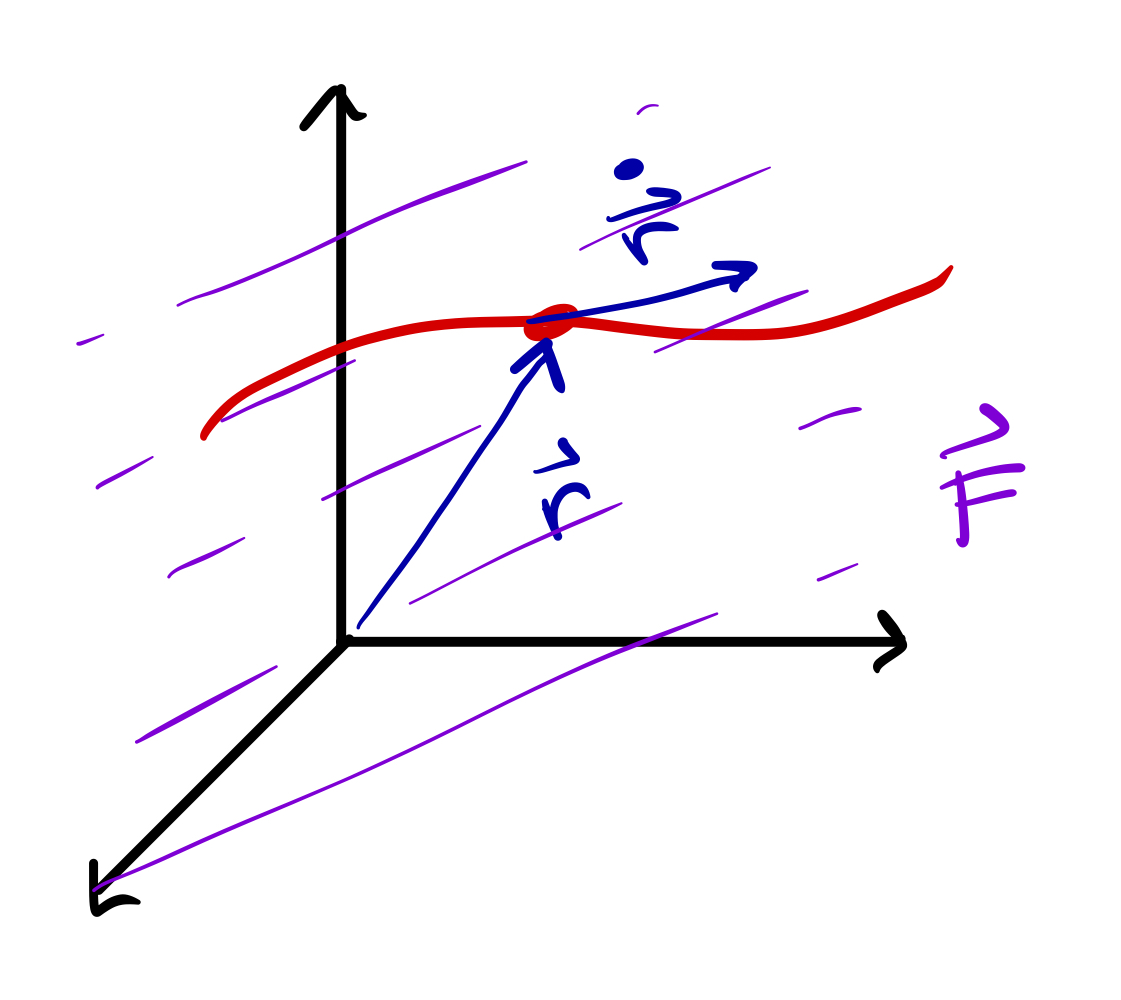
\includegraphics[width=1.0\linewidth]{2-particula} 
\end{wrapfigure}

la cual corresponde a una ecuación diferencial de segundo orden que estará completamente determinada por la fuerza y las condiciones iniciales para la posición $\vec{r}(0)$ y la velocidad $\dot{\vec{r}}(0)$. Luego, el sistema es \textit{determinista}, dado que solo con las condiciones iniciales, podemos determinar el estado del sistema en todo tiempo.


Ahora, si consideramos la descripción de la dinámica a partir de la mecánica analítica, las ecuaciones de movimiento estarán dadas por las ecuaciónes de Euler-Lagrange,
\begin{equation}
  \dv{t}\left(\pdv{L}{\dot{q}^{i}}\right)-\pdv{L}{q^{i}}=0,\qquad L=L(q,\qd,t),\qquad i=1,...,N
\end{equation}
\begin{equation}
  \implies \pdv{L}{q^j}{\qd^{i}}\qd^j+\pdv{\qd^j}\left(\pdv{L}{\qd^{i}}\right)\ddot{q}^j-\pdv{L}{q^{i}}=0
\end{equation}
\begin{equation}
  \implies \left(\pdv{L}{\qd^j}{\qd^{i}}\right)\ddot{q}^j=\pdv{L}{q^{i}}-\pdv{L}{q^j}{\qd^{i}}\qd^j 
\end{equation}
ó
\begin{equation}
 W_{ij}(q,\qd )\ddot{q}^j=\pdv{L}{q^{i}}-\pdv{L}{q^j}{\qd^{i}}\qd^j 
\end{equation}
donde
\begin{equation}
  W_{ij}=\pdv{L}{\qd^j}{\qd^{i}}
\end{equation}
es conocida como la \textit{matriz Hessiana}.

Podríamos concluir que cuando exsten simetrías de gauge, entonces $\det (W)=0$. Este tipo de sistemas son conocidos como \textit{sistemas singulares}.

\begin{ej}
	Consideremos el siguiente Lagrangeano:
	\begin{equation}
  L(q,\qd )=\frac{1}{2}\dot{x}^2+\dot{x}y+\frac{1}{2}(x-y)^2
\end{equation}
entonces $N=2$, donde las coordenadas generaliadas y las velocidades generalizadas son
\begin{equation}
  q^{i}=(x,y),\qquad \qd^{i}=(\dot{x},\dot{y})
\end{equation}
La matriz Hessiana viene dada por
\begin{equation}
  W_{ij}=\mqty(\dfrac{\partial^2L}{\partial\dot{x}\partial\dot{x}} &&&\dfrac{\partial^2L}{\partial\dot{x}\partial\dot{y}} \\\\\dfrac{\partial^2L}{\partial\dot{y}\partial\dot{x}} &&&\dfrac{\partial^2L}{\partial\dot{y}\partial\dot{y}} )=\mqty(1&0\\0&0)
\end{equation}
luego, $\det(W)=0$.

Entonces, podemos afirmar que este Lagrangeano posee simetrías locales (dinámica no determinista). Por inspección, consideremos 
\begin{align}
  \d_sx=\epsilon_1(t),\qquad \d_sy=\epsilon_2(t)
\end{align}
Luego, 
\begin{align}
  \d_sL&=\dot{x}\dot{\epsilon}_1+\dot{\epsilon}_1y+\dot{x}\epsilon_2+(x-y)\epsilon_1-(x-y)\epsilon_2 + \underbrace{\textcolor{blue}{\dot{x}\epsilon_1+x\dot{\epsilon}_1-\dot{x}\epsilon_1-x\dot{\epsilon}_1}}_{\textcolor{blue}{=0}}\\
  &=(\dot{x}+y-x)\dot{\epsilon}_1+(\dot{x}+y-x)\epsilon_2-(\dot{x}+y-x)\epsilon_1+\dv{t}(x\epsilon_1)\\
  &=(\dot{x}+y-x)(\dot{\epsilon}_1+\epsilon_2-\epsilon_1)+\dv{t}(x\epsilon_1)
\end{align}
Por lo tanto, la acción es invariante si
\begin{equation}
\boxed{  \epsilon_2=\epsilon_1-\dot{\epsilon}_1}
\end{equation}
Este ejemplo es ilustrativo para mostrar que
\begin{tcolorbox}
	\begin{equation}
		\text{Simetrías internas}\implies\text{Lagrangeano singular}
	\end{equation}
\end{tcolorbox}
\end{ej}

El punto de partida para el formalismo Hamiltoniano es definir los momentos canónicos, dados por
\begin{equation}
  p_i=\pdv{L}{\qd^{i}}
\end{equation}
Consideremos ahora un sistema gobernado por un Lagrangeano de la forma
\begin{equation}
  L=\frac{1}{2}\sum_{i,j=1}^NW_{ij}(q)\qd^{i}\qd^{j}+\sum_i^N\eta_i(q)\qd^{i}-V(q)
\end{equation}
Los momentos canónicos estan dados por
\begin{equation}\label{2.star}
  p_i=\sum_{j}W_{ij}(q)\qd^j+\eta_i(q)
\end{equation}
Consideremos el caso donde $W$ es singular y de rango $R_W$, esta posee $N-R_W$ autovectores asociados al autovalor nulo $\vec{v}_{(\a) }$ con $\a=1,...,N-R_W$.

De \eqref{2.star}, tenemos que
\begin{equation}
  \sum_i v_{(\a) }^{i}W_{ij}(q)=0
\end{equation}
entonces
\begin{equation}
  \sumi \vec{v}_{(\a) }^{i}(q)(p_i-\eta_i(q))=0\qquad (\text{Vínculos $N-R_W$})
\end{equation}
Ahora, llamamos $\{p_a\}$ al conjunto de $R_W$ momenta linalmente independientes, y al conjunto restante $(N-R_W)$ momenta los llamamos $\{p_\a \}$. Entonces la ecuación de los vínculos será
\begin{equation}
  \sum_\b M_\a ^{~\b }(q)p_\b -F_\a (q,\{p_a\})=0
\end{equation}
con
\begin{equation}
  M_\a ^{~\b }(q)=v_{(\a )}^{~\b }(q)
\end{equation}
y
\begin{equation}
  F_\a (q,\{p_a\}) =\sumi v_{(\a )}^{i }\eta_i(q)-\sum_bv_{(\a )}^{b }(q)p_b
\end{equation}
Necesariamente $M$ es una matriz invertible, puesto que de lo contrario habrían más vínculos. 
Puesto que $\det(M)\neq 0$, los vínculos pueden ser escritos en su forma estándar,
\begin{equation}
  \f_\a (p,q)=p_\a -g_\a (q,\{p_a\})=0
\end{equation}
donde
\begin{equation}
  g_\a =\sum_\b (M^{-1})_\a ^{~\b }F_\b (q,\{p_a\})
\end{equation}
Estos son conocidos como \textit{vínculos primarios}, puesto que se obtienen a partir de la definición de las momenta, sin utilizar las ecuaciones de movimiento.

Es el $2N$-espacio de fase, los vínculos definen sub-espacio $\Gamma_p $ de dimensión $2N-(N-R_W)=N+R_W$.

Para poder aplicar el mecanismo de Dirac es fundamental identificar el número exacto de vínculos en la teoría. Esto implica que los vínculos sean funcionalmente independientes y que el número d vínculos sea constante a lo largo del espacio de fase. La región del espacio de fase que satisface estas condiciones es conocida como \textit{sector canónico} de la teoría. Por lo tanto, los sectores canónicos cumplen con:
\begin{enumerate}
	\item condiciones de regularidad, y
	\item condiciones de no degenarción.
\end{enumerate}

%\subsection{Condición de regularidad}
%Si llamamos $z^{i}\equiv (q,p)$ con $i=1,...,2N$ son las coordenadas del espacio de fase $\G $, los vínculos $\f^\a =0$, donde $\a=1,...,M$ definen la superficie de vínculos $\G_p$, la cual viene dada por
%\begin{equation}
%  \G_p=\{\bar{z}\in \G \, |\,  \f^\a(\bar{z})=0, \quad \a=1,...,M <2N\}
%\end{equation}





































\newpage
\section{Clase 3}
\subsection{Dependencia funcional*}
Sea $D\subset  \mathbb{R}^N$ un conjunto abierto y consideremos $m$ funciones reales de clase $C^1$ en $D$,
\begin{align}
  u_1&=f_1(x_1,..,x_n)\\
  \vdots\\
  u_m&=f_m(x_1,..,x_n)
\end{align}
Se dice que las funciones $f_i$ con $i=1,...,m$ son dependientes en el conjunto, si existe una función real $F:S\rightarrow \mathbb{R}$ de clase $C^1$ en un conjunto abierto $S\subset  \mathbb{R}^m$ que incluye $f_1(D)\times f_2(D)\times \cdots \times f_m(D)$, que no se anule en ningún entorno completo de $S$ y tal que
\begin{equation}
  F[f_1(x_1,...,x_n),...,f_m(x_1,...,x_n)]=0, \quad \forall (x_1,...,x_n)\in D
\end{equation}
También diremos que si $f_k(x_1,...,x_n)$ es una de las funciones dadas, depende funcionalmente de las otras funciones $f_i$ con $i=1,...,m$ y $i\neq k$ si existe una función $\varphi$ de clase $C^1$ tal que
\begin{equation}
  f_k(x_1,...,x_n)=\varphi[f_1(x_1,...,x_n),...,f_{k-1},f_{k+1},...,f_k]
\end{equation}
Las funciones se dicen independientes funcionalmente, si no son dependientes funcionalmente.

\begin{ej}
	Sea $f$ y $g$ don funciones de clase $C^1$ en un abierto $D\subset \mathbb{R}^2$. Si $g$ depende funcionalmente de $f$, entonces
	\begin{equation}
  g(x,y)=\varphi[f(x,y)],\quad \forall x,y\in D.
\end{equation}
Podemos reescribir esto como
\begin{equation}
  \varphi[f(x,y)]- g(x,y)=0
\end{equation}
Derivando a ambos lados con respecto a $x$
\begin{equation}
  \varphi'\pdv{f}{x}-\pdv{g}{x}=0
\end{equation}
y con respecto a $y$
\begin{equation}
  \varphi'\pdv{f}{y}-\pdv{g}{y}=0
\end{equation}
Lo que permite escribir el sistema como
\begin{equation}
  \mqty(\pdv{f}{x}&&\pdv{g}{x}\\\\ \pdv{f}{y}&&\pdv{g}{y})\mqty(\varphi'\\\\-1)=0,\qquad \varphi'\equiv \pdv{\varphi}{f}
\end{equation}
Dado que el sistema tiene solución no trivial, implica que el determinante de la matriz anterior se debe anular, es decir,
\begin{equation}
   \mqty|\pdv{f}{x}&&\pdv{g}{x}\\\\ \pdv{f}{y}&&\pdv{g}{y}|=0
\end{equation}
Una condición necesaria para que ocurra dependencia funcional es que el Jacobiano se anule,
\begin{equation}
  \pdv{(f,g)}{(x,y)}=0,\quad \forall (x,y)\in D.
\end{equation}
\end{ej}

\begin{ej}
	Dependencia funcional. Consideremos las siguientes funciones
	\begin{align}
  u(x,y)&=e^{2x-y}\\
  v(x,y)&=e^{2y-4x}
\end{align}
\begin{equation}
  \implies F(u,v)=u^2v-1,\qquad v=\frac{1}{u^2}=\varphi(u)
\end{equation}
\begin{equation}
  \implies \pdv{(u,v)}{(x,y)}=\mqty|2e^{2x-y}&&-4e^{2y-4x}\\\\ -e^{2x-y}&&2e^{2y-4x}|=0
\end{equation}
Luego, son funcionalmente dependientes.
\end{ej}






\subsection{Condiciones de regularidad}
Si llamamos $z^{i}\equiv (q,p)$ con $i=1,...,2N$ son las coordenadas del espacio de fase $\G $, los vínculos $\f^\a =0$, donde $\a=1,...,R$ definen la superficie de vínculos $\bar{\G}$, la cual viene dada por
\begin{equation}
  \bar{\G}=\{\bar{z}\in \G \, |\,  \f^\a(\bar{z})=0, \quad \a=1,...,R\leq 2N\}
\end{equation}
Los vínculos $\f_\a=0$ son regulares si y sólo si sus pequeñas variaciones evaluadas sobre $\bar{\G}$ son $R$ funciones linealmente independientes de $\d z^{i}$. A primer orden en $\d z^{i}$, la variación de los vínculos será $\d\f_\a=J_{\a i}\d z^{i}$ donde $J_{\a i}=\eval{\pdv{\f_\a }{z^{i}}}_{\bar{\G }}$. El conjunto de los vínculos $\f_\a =0$ es regular si y sólo si el Jacobiano $J$ tiene rango máximo, es decir, $\text{Rang}(J)=R$.

\begin{ej}
	Consideremos lo siguientes vínculos
	\begin{equation}
  \f^1=q=0,\qquad \f^2=pq=0
\end{equation}
El Jacobiano es
\begin{equation}
  J=\mqty|1&&p\\0&&q|_{\bar{\G }}=\mqty|1&&p\\0&&0|
\end{equation}
\begin{equation}
  \implies \text{Rang}(J)=1
\end{equation}
Luego, los vínculos son funcionalmente dependientes, dado que $R=2$.
\end{ej}

Cuando los vínculos saisfacen las condiciones de regularidad, se cumplen los siguientes teoremas:
\begin{teor}\label{teo:1}
	Si una función $G$ del espacio de fase se anula en la superficie de los vínculos $\f_\a =0$, entonces $G=f^\a \f_\a $ para alguna función $g^\a $.
\end{teor}

\begin{teor}\label{teo:2}
	Si $\lambda_n \d q^n+\m ^n \d p_n=0$ para variaciones arbitrarias $\d q^n$ y $\d p_n$ tangentes a la superficie de los vínculos, entonces
	\begin{align}
  \lambda_n &=u^m \pdv{\f_m }{q^n }\\
  \m^n  &=u^m\pdv{\f_m }{p_n }
\end{align}
Para algún $u^m $. Las igualdades se satisfacen en la superficie de los vínculos \footnote{La demostración de este Teorema se puede ver en \cite{Henneaux:1994lbw}.}.
\end{teor}

Cuando tenemos vínculos, el mapeo $(q^n, \qd ^n)\rightarrow (p_n,q^n)$ no es unívoco dado que mapeo puntos desde una $2N$-variedad a una $(2N-R)$-variedad ($\G \rightarrow \bar{\G }$). Por lo tanto, las imágenes inversas de un punto dado de $\f_\a =0$ forma una vaiedad $R$-dimensional.

\begin{ej}
	Consideremos el siguiente Lagrangeano
	\begin{equation}
  L=\frac{1}{2}(\qd ^1-\qd^2)^2
\end{equation}
Las momenta vienen dadas por
\begin{align}
  p_1&=\qd^1-\qd^2\\
  p_2&=\qd^2-\qd^1
\end{align}
Notamos que tenemos una superficie de vínculos dada por
\begin{equation}
  \f =p_1+p_2=0
\end{equation}
Todos los puntos $\qd^2-\qd^1=c$ son mapeados a un único punto en el espacio de fase $p_1=-c=-p_2$.
%TODO img


\end{ej}


Con el fin de que la transformación sea uni-valuada es necsario introducir parámetros extras que indiquen la localización de $\qd$ en la variedad inversa. Estos parámetros podrían ser pensados como coordenadas en la variedad inversa para algún punto $P_n$.

\subsection{Mecanismo de Dirac para sistemas con vínculos}
Para continuar con la descripción dinámica sebemos tener el Hamiltoniano del sistema, el cual, en general, viene dado por
\begin{equation}
  H=p_n\qd^n -L(q^n,\qd^n,t)
\end{equation}
Si calculamos la variación de $H$, se tiene
\begin{align}
  \d H&=\d p_n\qd^n +p_n\d \qd^n -\underbrace{\pdv{L}{\qd^n }}_{p_n}\d \qd^n -\pdv{L}{q^n }\d ^n \\
  &=\d p_n \qd ^n -\pdv{L}{q^n }\d q^n  \label{3.1}
\end{align}
Luego, $H=H(p^n ,q_n)$. Esto es cierto cuando el sistema no tiene vínculos. 

En un sistema con vínculos, este Hamiltoniano no está únicamente determinado como función de los $p^n $ y $q_n $. Esto puede ser notado, dado que $\d p_n $ en la superficie de los vínculos no son todos independientes, sino que están restringidos a satisfacer los vínculos. Estos $\f_\a $ son identidades cuando los $p_n $ son expresados en función de $\qd^n $ y $q^n$ por medio de la transformación de Legendre. Por lo tanto, el Hamiltoniano canónico está sólo bien definido en la sub-variedad definida por los vínculos primarios.

De \eqref{3.1} tenemos que
\begin{align}
  \pdv{H}{p_n}\d p_n+\pdv{H}{q^n }\d q^n &=\d p_n \qd^n -\pdv{L}{q^n }\d q^n 
\end{align}
\begin{align}
  \implies \left(\pdv{H}{p_n }-\qd^n \right)\d p_n +\left(\pdv{H}{q^n}+\pdv{L}{q^n }\right)\d q^n =0
\end{align}
A partir del Teorema \ref{teo:2} tenemos que
\begin{align}
  \qd^n &=\pdv{H}{p_n }+u^m \pdv{\f_m}{p_n}
\end{align}

\subsection{Principio de acción para el Hamiltoniano con vínculos}
Para el caso de sistemas singulares es necesario introducir la información de los vínculos en el principio de acción. Esto lo haremos por medio de funciones aribitrarias (multiplicadores de Lagrange) de tal manera que nos entregue las ecuaciones de movimiento correctas. Para esto, definimos el \textit{Hamiltoniano primario}, el cual viene dado por
\begin{equation}
  H_p=H_c+u^\a \f_\a 
\end{equation}
Por lo tanto, la acción vendrá dada por
\begin{align}
  I[q^n,p_n,u^\a  ]=\int(\qd^n p_n-H_c-u^\a \f_\a )\dd t
\end{align}
Las ecuaciones de movimiento vienen dadas por
\begin{equation}
\begin{split}
  &\qd^n =\pdv{H_p}{p_n }=\pdv{H_c}{p_n }+u^\a \pdv{\f_\a }{p_n }\\
  &\dot{p}=-\pdv{H_p}{q^n }=-\pdv{H_c}{q^n}-u^\a \pdv{\f_\a }{q^n }\\
 &\f_\a =0
\end{split}
\end{equation}


















































\newpage
\section{Clase 4}
%\subsection{* Interludio de la clase pasada}
De la clase pasada habíamos afirmado que el conjunto $\f^r=0$ es regular si y sólo si el Jacobiano $J_i^r\equiv \eval{\pdv{\f^r}{z^{i}}}_\G $ tiene rango máximo, es decir, $\text{Rango}(J)=R$. 

\begin{teor}	\textbf{(Teorema del rango constante)}
\begin{equation}
u=f(x)=\left\{\begin{array}{ll}
  u_1&=f_1(x_1,..,x_n)\\
  &\vdots\\
  u_m&=f_m(x_1,..,x_n)
\end{array}
\right.
\end{equation}
\begin{equation}
  J(f(x))=\left(\pdv{f}{x}\right)
\end{equation}
La matriz Jacobiana $Jf(x)$ tenga un rango máximo igual a $r$, con $0<r\leq m$.
\begin{itemize}
	\item Todos los menores de orden  mayor que $r$
	\item Para cada $r\in D$, existe un menor de orden $r$ en donde $Jf$ es nulo.
\end{itemize}
Entonces:
\begin{enumerate}
	\item Existen $r$ funciones $f_i$ independientes,
	\item Cada una de las $m-r$ funciones restantes dependen de las funciones independientes.
\end{enumerate}
\end{teor}

Al final de la clase pasada hicimos dos afirmaciones:
\begin{Propo}
	Sobre el subespacio $\G_p$ definidos $\Phi_\a (p,q)=0$, el Hamiltoniano canónico sólo depende de de $\{q_i\}$, $\{p_j\}$ independientes.
\end{Propo}
\begin{Propo}
	Las ecuaciones de Hamilton serán 
	\begin{equation}
\begin{split}
  &\qd^n =\pdv{H_p}{p_n }=\pdv{H_c}{p_n }+u^\a \pdv{\f_\a }{p_n }\\
  &\dot{p}=-\pdv{H_p}{q^n }=-\pdv{H_c}{q^n}-u^\a \pdv{\f_\a }{q^n }\\
 &\f_\a =0
\end{split}
\end{equation}
\end{Propo}

Para el caso b) aparecían nuevos vínculos ($X$) a los cuales nuevamente imponemos la preservación en el tiempo
\begin{equation}
  [X_a,H_c]+u^m[X_a,\f_m]=0
\end{equation}
Una vez finalizado el proceso, nos quedaremos con una serie de vínculos secundarios, que denotaremos
\begin{equation}
  \f_a=0;\qquad a=\underbrace{(N-R_w)}_s+1+\cdots + s+k
\end{equation}
donde $k$ es el número de vínculos secundarios y por lo tanto, el número total de vínculos será
\begin{equation}
  \Phi_j=0,\qquad j=1,...,s+k
\end{equation}

\subsection{Ecuaciones débiles y fuertes}
\begin{defi}
Vamos a introducir el símbolo de igualdad débil para las ecuaciones de los vínculos
\begin{equation}
  \f_j\approx 0
\end{equation}
Con esto enfatizamos que esta cantidad está numéricamente restringida a ser cero pero que no es idénticamente cero a lo largo de todo el espacio de fase. Esto significa en particular que los corchetes de Poisson con funciones dependientes de las variables canónicas no se anulan.

Más generalmente, dos funciones $F$ y $G$ que coinciden en la superficie de los vínculos, se dicen débilmente iguales $F\approx G$
\begin{equation}
  F\approx G\implies F-G=g^j\f_j
\end{equation}
\end{defi}

\subsection{Restricciones en los multiplicadores de Lagrange}
Suponemos que ya hemos encontrado todos los vínculos, entonces podemos pasar a estudiar las resticciones sobre los multiplicadores de Lagrange, las cuales serán de la forma
\begin{equation}\label{4.2}
  [\f_j,H_c]+u^m[\f_j,\f_m]\approx 0
\end{equation}
donde $m=1,...,s$ y $j=1,...,s+k$ y $s$ es el número de vínculos primarios. Podemos considerar a \eqref{4.2} como un conjunto de $k+s$ ecuaciones lineales con $s\leq s+k$ para $u^m$ con coeficientes que son funciones de $p$ y $q$.

La solución más general para \eqref{4.2} es 
\begin{equation}
  u^m=U^m+\n^m
\end{equation}
donde $U^m$ es una solución particular de \eqref{4.2} y $\n^m $ es la solución homogénea de \eqref{4.2}, es decir,
\begin{equation}
  \n^\m [\f_j,\f_m]\approx 0.
\end{equation}



















% Bibliography

%% [A] Recommended: using JHEP.bst file
%% \bibliographystyle{JHEP}
%% \bibliography{biblio.bib}

%% or
%% [B] Manual formatting (see below)
%% (i) We suggest to always provide author, title and journal data or doi:
%% in short all the informations that clearly identify a document.
%% (ii) please avoid comments such as "For a review'', "For some examples",
%% "and references therein" or move them in the text. In general, please leave only references in the bibliography and move all
%% accessory text in footnotes.
%% (iii) Also, please have only one work for each \bibitem.

\newpage
\bibliographystyle{JHEP}
\bibliography{biblio.bib}
\end{document}
